\documentclass[twoside]{book}

% Packages required by doxygen
\usepackage{fixltx2e}
\usepackage{calc}
\usepackage{doxygen}
\usepackage[export]{adjustbox} % also loads graphicx
\usepackage{graphicx}
\usepackage[utf8]{inputenc}
\usepackage{makeidx}
\usepackage{multicol}
\usepackage{multirow}
\PassOptionsToPackage{warn}{textcomp}
\usepackage{textcomp}
\usepackage[nointegrals]{wasysym}
\usepackage[table]{xcolor}

% Font selection
\usepackage[T1]{fontenc}
\usepackage[scaled=.90]{helvet}
\usepackage{courier}
\usepackage{amssymb}
\usepackage{sectsty}
\renewcommand{\familydefault}{\sfdefault}
\allsectionsfont{%
  \fontseries{bc}\selectfont%
  \color{darkgray}%
}
\renewcommand{\DoxyLabelFont}{%
  \fontseries{bc}\selectfont%
  \color{darkgray}%
}
\newcommand{\+}{\discretionary{\mbox{\scriptsize$\hookleftarrow$}}{}{}}

% Page & text layout
\usepackage{geometry}
\geometry{%
  a4paper,%
  top=2.5cm,%
  bottom=2.5cm,%
  left=2.5cm,%
  right=2.5cm%
}
\tolerance=750
\hfuzz=15pt
\hbadness=750
\setlength{\emergencystretch}{15pt}
\setlength{\parindent}{0cm}
\setlength{\parskip}{3ex plus 2ex minus 2ex}
\makeatletter
\renewcommand{\paragraph}{%
  \@startsection{paragraph}{4}{0ex}{-1.0ex}{1.0ex}{%
    \normalfont\normalsize\bfseries\SS@parafont%
  }%
}
\renewcommand{\subparagraph}{%
  \@startsection{subparagraph}{5}{0ex}{-1.0ex}{1.0ex}{%
    \normalfont\normalsize\bfseries\SS@subparafont%
  }%
}
\makeatother

% Headers & footers
\usepackage{fancyhdr}
\pagestyle{fancyplain}
\fancyhead[LE]{\fancyplain{}{\bfseries\thepage}}
\fancyhead[CE]{\fancyplain{}{}}
\fancyhead[RE]{\fancyplain{}{\bfseries\leftmark}}
\fancyhead[LO]{\fancyplain{}{\bfseries\rightmark}}
\fancyhead[CO]{\fancyplain{}{}}
\fancyhead[RO]{\fancyplain{}{\bfseries\thepage}}
\fancyfoot[LE]{\fancyplain{}{}}
\fancyfoot[CE]{\fancyplain{}{}}
\fancyfoot[RE]{\fancyplain{}{\bfseries\scriptsize Generated by Doxygen }}
\fancyfoot[LO]{\fancyplain{}{\bfseries\scriptsize Generated by Doxygen }}
\fancyfoot[CO]{\fancyplain{}{}}
\fancyfoot[RO]{\fancyplain{}{}}
\renewcommand{\footrulewidth}{0.4pt}
\renewcommand{\chaptermark}[1]{%
  \markboth{#1}{}%
}
\renewcommand{\sectionmark}[1]{%
  \markright{\thesection\ #1}%
}

% Indices & bibliography
\usepackage{natbib}
\usepackage[titles]{tocloft}
\setcounter{tocdepth}{3}
\setcounter{secnumdepth}{5}
\makeindex

% Hyperlinks (required, but should be loaded last)
\usepackage{ifpdf}
\ifpdf
  \usepackage[pdftex,pagebackref=true]{hyperref}
\else
  \usepackage[ps2pdf,pagebackref=true]{hyperref}
\fi
\hypersetup{%
  colorlinks=true,%
  linkcolor=blue,%
  citecolor=blue,%
  unicode%
}

% Custom commands
\newcommand{\clearemptydoublepage}{%
  \newpage{\pagestyle{empty}\cleardoublepage}%
}

\usepackage{caption}
\captionsetup{labelsep=space,justification=centering,font={bf},singlelinecheck=off,skip=4pt,position=top}

%===== C O N T E N T S =====

\begin{document}

% Titlepage & ToC
\hypersetup{pageanchor=false,
             bookmarksnumbered=true,
             pdfencoding=unicode
            }
\pagenumbering{alph}
\begin{titlepage}
\vspace*{7cm}
\begin{center}%
{\Large My Project }\\
\vspace*{1cm}
{\large Generated by Doxygen 1.8.13}\\
\end{center}
\end{titlepage}
\clearemptydoublepage
\pagenumbering{roman}
\tableofcontents
\clearemptydoublepage
\pagenumbering{arabic}
\hypersetup{pageanchor=true}

%--- Begin generated contents ---
\chapter{R\+E\+A\+D\+ME}
\label{md__r_e_a_d_m_e}
\Hypertarget{md__r_e_a_d_m_e}
CS 3560 Term Project Repository

Game\+: Checkers

Jordan Ward \href{mailto:jw363912@ohio.edu}{\tt jw363912@ohio.\+edu}

Nic Gill \href{mailto:ng344516@ohio.edu}{\tt ng344516@ohio.\+edu}

Mackenzie Schnaekel \href{mailto:ms840314@ohio.edu}{\tt ms840314@ohio.\+edu}

Dashaun Slaughter \href{mailto:ds946041@ohio.edu}{\tt ds946041@ohio.\+edu}

Chase Gindlesperger \href{mailto:cg197415@ohio.edu}{\tt cg197415@ohio.\+edu} 
\chapter{Hierarchical Index}
\section{Class Hierarchy}
This inheritance list is sorted roughly, but not completely, alphabetically\+:\begin{DoxyCompactList}
\item \contentsline{section}{main\+\_\+savitch\+\_\+14\+:\+:game}{\pageref{classmain__savitch__14_1_1game}}{}
\begin{DoxyCompactList}
\item \contentsline{section}{main\+\_\+savitch\+\_\+14\+:\+:checkers}{\pageref{classmain__savitch__14_1_1checkers}}{}
\end{DoxyCompactList}
\item \contentsline{section}{main\+\_\+savitch\+\_\+14\+:\+:space}{\pageref{classmain__savitch__14_1_1space}}{}
\end{DoxyCompactList}

\chapter{Class Index}
\section{Class List}
Here are the classes, structs, unions and interfaces with brief descriptions\+:\begin{DoxyCompactList}
\item\contentsline{section}{\hyperlink{classmain__savitch__14_1_1checkers}{main\+\_\+savitch\+\_\+14\+::checkers} }{\pageref{classmain__savitch__14_1_1checkers}}{}
\item\contentsline{section}{\hyperlink{classmain__savitch__14_1_1game}{main\+\_\+savitch\+\_\+14\+::game} }{\pageref{classmain__savitch__14_1_1game}}{}
\item\contentsline{section}{\hyperlink{classmain__savitch__14_1_1space}{main\+\_\+savitch\+\_\+14\+::space} }{\pageref{classmain__savitch__14_1_1space}}{}
\end{DoxyCompactList}

\chapter{Class Documentation}
\hypertarget{classmain__savitch__14_1_1checkers}{}\section{main\+\_\+savitch\+\_\+14\+:\+:checkers Class Reference}
\label{classmain__savitch__14_1_1checkers}\index{main\+\_\+savitch\+\_\+14\+::checkers@{main\+\_\+savitch\+\_\+14\+::checkers}}
Inheritance diagram for main\+\_\+savitch\+\_\+14\+:\+:checkers\+:\begin{figure}[H]
\begin{center}
\leavevmode
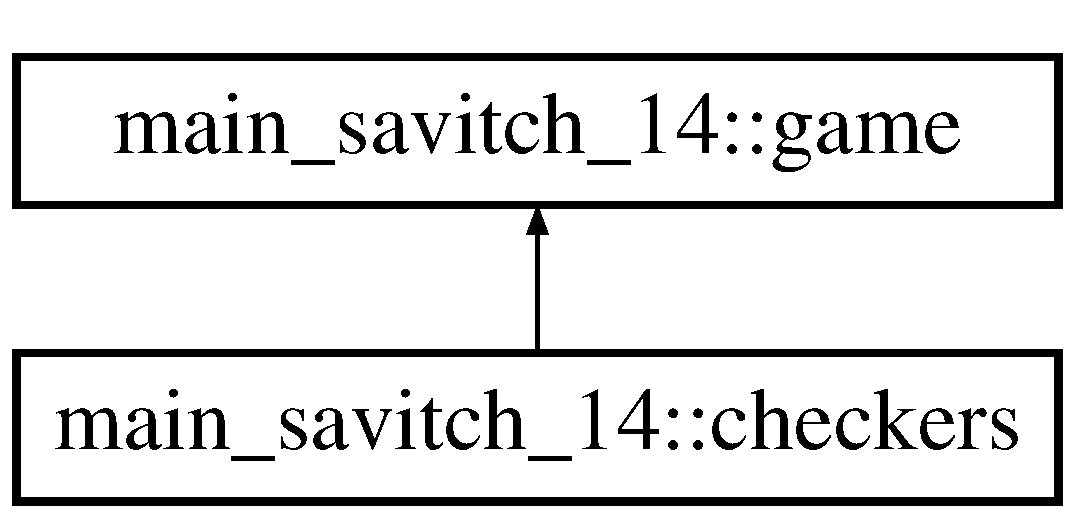
\includegraphics[height=2.000000cm]{classmain__savitch__14_1_1checkers}
\end{center}
\end{figure}
\subsection*{Public Member Functions}
\begin{DoxyCompactItemize}
\item 
bool \hyperlink{classmain__savitch__14_1_1checkers_afc7d56fe1f0637a02cad352e9cda9ee3}{is\+\_\+legal} (const string \&move) const
\item 
int \hyperlink{classmain__savitch__14_1_1checkers_a1705b4e1bfe04205ebb7703925b50f9f}{evaluate} () const
\item 
void \hyperlink{classmain__savitch__14_1_1checkers_a8a08c0555d5b8c264472cc94a2f007e3}{make\+\_\+move} (const string \&move)
\item 
void \hyperlink{classmain__savitch__14_1_1checkers_aa4b4867ee171d04f5473f4ca38a9729a}{compute\+\_\+moves} (queue$<$ string $>$ \&moves) const
\item 
\mbox{\Hypertarget{classmain__savitch__14_1_1checkers_aa99f69ed300d81b6340f87b59ebba031}\label{classmain__savitch__14_1_1checkers_aa99f69ed300d81b6340f87b59ebba031}} 
void {\bfseries display\+\_\+status} () const
\item 
\mbox{\Hypertarget{classmain__savitch__14_1_1checkers_a716b963325b1455e63c25afe89d617d9}\label{classmain__savitch__14_1_1checkers_a716b963325b1455e63c25afe89d617d9}} 
\hyperlink{classmain__savitch__14_1_1game}{game} $\ast$ {\bfseries clone} () const
\item 
bool \hyperlink{classmain__savitch__14_1_1checkers_ab8481b1a443f4b190d3ff508ab6f62a7}{is\+\_\+game\+\_\+over} () const
\item 
void \hyperlink{classmain__savitch__14_1_1checkers_ad3ee0adbdabda9136ecd46b958c83d24}{restart} ()
\item 
game\+::who \hyperlink{classmain__savitch__14_1_1checkers_aad9a08662e9fdf62752c60997b29370e}{winning} () const
\end{DoxyCompactItemize}
\subsection*{Additional Inherited Members}


\subsection{Member Function Documentation}
\mbox{\Hypertarget{classmain__savitch__14_1_1checkers_aa4b4867ee171d04f5473f4ca38a9729a}\label{classmain__savitch__14_1_1checkers_aa4b4867ee171d04f5473f4ca38a9729a}} 
\index{main\+\_\+savitch\+\_\+14\+::checkers@{main\+\_\+savitch\+\_\+14\+::checkers}!compute\+\_\+moves@{compute\+\_\+moves}}
\index{compute\+\_\+moves@{compute\+\_\+moves}!main\+\_\+savitch\+\_\+14\+::checkers@{main\+\_\+savitch\+\_\+14\+::checkers}}
\subsubsection{\texorpdfstring{compute\+\_\+moves()}{compute\_moves()}}
{\footnotesize\ttfamily void main\+\_\+savitch\+\_\+14\+::checkers\+::compute\+\_\+moves (\begin{DoxyParamCaption}\item[{queue$<$ string $>$ \&}]{moves }\end{DoxyParamCaption}) const}

Computes moves for the computer 
\begin{DoxyParams}{Parameters}
{\em queue$<$string$>$\&} & moves \\
\hline
\end{DoxyParams}
\begin{DoxyReturn}{Returns}
void 
\end{DoxyReturn}
\mbox{\Hypertarget{classmain__savitch__14_1_1checkers_a1705b4e1bfe04205ebb7703925b50f9f}\label{classmain__savitch__14_1_1checkers_a1705b4e1bfe04205ebb7703925b50f9f}} 
\index{main\+\_\+savitch\+\_\+14\+::checkers@{main\+\_\+savitch\+\_\+14\+::checkers}!evaluate@{evaluate}}
\index{evaluate@{evaluate}!main\+\_\+savitch\+\_\+14\+::checkers@{main\+\_\+savitch\+\_\+14\+::checkers}}
\subsubsection{\texorpdfstring{evaluate()}{evaluate()}}
{\footnotesize\ttfamily int main\+\_\+savitch\+\_\+14\+::checkers\+::evaluate (\begin{DoxyParamCaption}{ }\end{DoxyParamCaption}) const\hspace{0.3cm}{\ttfamily [virtual]}}

returns who is currently winning based on the number of chips \begin{DoxyReturn}{Returns}
int 
\end{DoxyReturn}


Implements \hyperlink{classmain__savitch__14_1_1game}{main\+\_\+savitch\+\_\+14\+::game}.

\mbox{\Hypertarget{classmain__savitch__14_1_1checkers_ab8481b1a443f4b190d3ff508ab6f62a7}\label{classmain__savitch__14_1_1checkers_ab8481b1a443f4b190d3ff508ab6f62a7}} 
\index{main\+\_\+savitch\+\_\+14\+::checkers@{main\+\_\+savitch\+\_\+14\+::checkers}!is\+\_\+game\+\_\+over@{is\+\_\+game\+\_\+over}}
\index{is\+\_\+game\+\_\+over@{is\+\_\+game\+\_\+over}!main\+\_\+savitch\+\_\+14\+::checkers@{main\+\_\+savitch\+\_\+14\+::checkers}}
\subsubsection{\texorpdfstring{is\+\_\+game\+\_\+over()}{is\_game\_over()}}
{\footnotesize\ttfamily bool main\+\_\+savitch\+\_\+14\+::checkers\+::is\+\_\+game\+\_\+over (\begin{DoxyParamCaption}{ }\end{DoxyParamCaption}) const\hspace{0.3cm}{\ttfamily [virtual]}}

Determines if the game is over \begin{DoxyReturn}{Returns}
bool 
\end{DoxyReturn}


Implements \hyperlink{classmain__savitch__14_1_1game}{main\+\_\+savitch\+\_\+14\+::game}.

\mbox{\Hypertarget{classmain__savitch__14_1_1checkers_afc7d56fe1f0637a02cad352e9cda9ee3}\label{classmain__savitch__14_1_1checkers_afc7d56fe1f0637a02cad352e9cda9ee3}} 
\index{main\+\_\+savitch\+\_\+14\+::checkers@{main\+\_\+savitch\+\_\+14\+::checkers}!is\+\_\+legal@{is\+\_\+legal}}
\index{is\+\_\+legal@{is\+\_\+legal}!main\+\_\+savitch\+\_\+14\+::checkers@{main\+\_\+savitch\+\_\+14\+::checkers}}
\subsubsection{\texorpdfstring{is\+\_\+legal()}{is\_legal()}}
{\footnotesize\ttfamily bool main\+\_\+savitch\+\_\+14\+::checkers\+::is\+\_\+legal (\begin{DoxyParamCaption}\item[{const string \&}]{move }\end{DoxyParamCaption}) const}

This function determines if a move is legal or illegal 
\begin{DoxyParams}{Parameters}
{\em const} & string\& move \\
\hline
\end{DoxyParams}
\begin{DoxyReturn}{Returns}
bool 
\end{DoxyReturn}
\mbox{\Hypertarget{classmain__savitch__14_1_1checkers_a8a08c0555d5b8c264472cc94a2f007e3}\label{classmain__savitch__14_1_1checkers_a8a08c0555d5b8c264472cc94a2f007e3}} 
\index{main\+\_\+savitch\+\_\+14\+::checkers@{main\+\_\+savitch\+\_\+14\+::checkers}!make\+\_\+move@{make\+\_\+move}}
\index{make\+\_\+move@{make\+\_\+move}!main\+\_\+savitch\+\_\+14\+::checkers@{main\+\_\+savitch\+\_\+14\+::checkers}}
\subsubsection{\texorpdfstring{make\+\_\+move()}{make\_move()}}
{\footnotesize\ttfamily void main\+\_\+savitch\+\_\+14\+::checkers\+::make\+\_\+move (\begin{DoxyParamCaption}\item[{const string \&}]{move }\end{DoxyParamCaption})}

Allows for a move to be made 
\begin{DoxyParams}{Parameters}
{\em const} & string\& move \\
\hline
\end{DoxyParams}
\begin{DoxyReturn}{Returns}
void 
\end{DoxyReturn}
\mbox{\Hypertarget{classmain__savitch__14_1_1checkers_ad3ee0adbdabda9136ecd46b958c83d24}\label{classmain__savitch__14_1_1checkers_ad3ee0adbdabda9136ecd46b958c83d24}} 
\index{main\+\_\+savitch\+\_\+14\+::checkers@{main\+\_\+savitch\+\_\+14\+::checkers}!restart@{restart}}
\index{restart@{restart}!main\+\_\+savitch\+\_\+14\+::checkers@{main\+\_\+savitch\+\_\+14\+::checkers}}
\subsubsection{\texorpdfstring{restart()}{restart()}}
{\footnotesize\ttfamily void main\+\_\+savitch\+\_\+14\+::checkers\+::restart (\begin{DoxyParamCaption}{ }\end{DoxyParamCaption})\hspace{0.3cm}{\ttfamily [virtual]}}

Resets the move number back to zero 

Reimplemented from \hyperlink{classmain__savitch__14_1_1game_ad521a7d78e7c163a0bc28b709f0d45fd}{main\+\_\+savitch\+\_\+14\+::game}.

\mbox{\Hypertarget{classmain__savitch__14_1_1checkers_aad9a08662e9fdf62752c60997b29370e}\label{classmain__savitch__14_1_1checkers_aad9a08662e9fdf62752c60997b29370e}} 
\index{main\+\_\+savitch\+\_\+14\+::checkers@{main\+\_\+savitch\+\_\+14\+::checkers}!winning@{winning}}
\index{winning@{winning}!main\+\_\+savitch\+\_\+14\+::checkers@{main\+\_\+savitch\+\_\+14\+::checkers}}
\subsubsection{\texorpdfstring{winning()}{winning()}}
{\footnotesize\ttfamily game\+::who main\+\_\+savitch\+\_\+14\+::checkers\+::winning (\begin{DoxyParamCaption}{ }\end{DoxyParamCaption}) const\hspace{0.3cm}{\ttfamily [virtual]}}

returns who is currently winning \begin{DoxyReturn}{Returns}
game 
\end{DoxyReturn}


Reimplemented from \hyperlink{classmain__savitch__14_1_1game_a2f0d5338c12bd98d52fe2383ece5c45e}{main\+\_\+savitch\+\_\+14\+::game}.



The documentation for this class was generated from the following files\+:\begin{DoxyCompactItemize}
\item 
checkers.\+h\item 
checkers.\+cc\end{DoxyCompactItemize}

\hypertarget{classmain__savitch__14_1_1game}{}\section{main\+\_\+savitch\+\_\+14\+:\+:game Class Reference}
\label{classmain__savitch__14_1_1game}\index{main\+\_\+savitch\+\_\+14\+::game@{main\+\_\+savitch\+\_\+14\+::game}}
Inheritance diagram for main\+\_\+savitch\+\_\+14\+:\+:game\+:\begin{figure}[H]
\begin{center}
\leavevmode
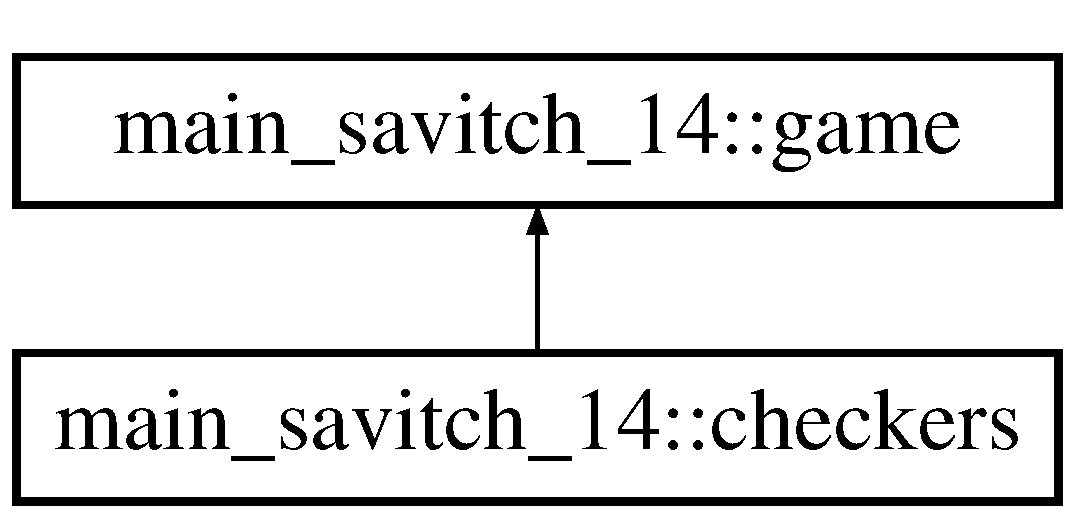
\includegraphics[height=2.000000cm]{classmain__savitch__14_1_1game}
\end{center}
\end{figure}
\subsection*{Public Types}
\begin{DoxyCompactItemize}
\item 
\mbox{\Hypertarget{classmain__savitch__14_1_1game_a4fe20fb287f809ae2b68e28e4ccba634}\label{classmain__savitch__14_1_1game_a4fe20fb287f809ae2b68e28e4ccba634}} 
enum {\bfseries who} \{ {\bfseries H\+U\+M\+AN}, 
{\bfseries N\+E\+U\+T\+R\+AL}, 
{\bfseries C\+O\+M\+P\+U\+T\+ER}
 \}
\end{DoxyCompactItemize}
\subsection*{Public Member Functions}
\begin{DoxyCompactItemize}
\item 
void \hyperlink{classmain__savitch__14_1_1game_a51e5d7be01076996b68449983874ff8f}{clear} () const
\item 
\hyperlink{classmain__savitch__14_1_1game_a65afffa6f5aa8dcd781ad38f898130e0}{game} ()
\begin{DoxyCompactList}\small\item\em Constructor for game class. \end{DoxyCompactList}\item 
\mbox{\Hypertarget{classmain__savitch__14_1_1game_a5e8d21d1d658a12db6fddacca3490671}\label{classmain__savitch__14_1_1game_a5e8d21d1d658a12db6fddacca3490671}} 
virtual \hyperlink{classmain__savitch__14_1_1game_a5e8d21d1d658a12db6fddacca3490671}{$\sim$game} ()
\begin{DoxyCompactList}\small\item\em Destructor for game class. \end{DoxyCompactList}\item 
who \hyperlink{classmain__savitch__14_1_1game_a4dbeaddb78059f7c5dcbf5cc4e026317}{play} ()
\end{DoxyCompactItemize}
\subsection*{Protected Member Functions}
\begin{DoxyCompactItemize}
\item 
virtual void \hyperlink{classmain__savitch__14_1_1game_ac58bfc07db8e604b07d2039b2cf7ab51}{display\+\_\+message} (const std\+::string \&message) const
\item 
virtual std\+::string \hyperlink{classmain__savitch__14_1_1game_af389f976b7a6c75e096990a09fac94ba}{get\+\_\+user\+\_\+move} ()
\item 
virtual who \hyperlink{classmain__savitch__14_1_1game_a5c1ab8b36fb977bbe9fe387e793e4ee5}{last\+\_\+mover} () const
\item 
virtual int \hyperlink{classmain__savitch__14_1_1game_a31dd5382cc6d64a6d58bcee55383cf1b}{moves\+\_\+completed} () const
\item 
virtual who \hyperlink{classmain__savitch__14_1_1game_a4e68409618474d19742dd5f75f92f5c9}{next\+\_\+mover} () const
\item 
virtual who \hyperlink{classmain__savitch__14_1_1game_a98469e89e13c73a5ee70407a2164888c}{opposite} (who player) const
\item 
virtual who \hyperlink{classmain__savitch__14_1_1game_a2f0d5338c12bd98d52fe2383ece5c45e}{winning} () const
\item 
virtual void \hyperlink{classmain__savitch__14_1_1game_a20597d0caa907aea47b27fed8be3759b}{make\+\_\+move} (const std\+::string \&move)
\item 
virtual void \hyperlink{classmain__savitch__14_1_1game_ad521a7d78e7c163a0bc28b709f0d45fd}{restart} ()
\item 
\mbox{\Hypertarget{classmain__savitch__14_1_1game_a7b663057f59210dd52738facfc40d959}\label{classmain__savitch__14_1_1game_a7b663057f59210dd52738facfc40d959}} 
virtual \hyperlink{classmain__savitch__14_1_1game}{game} $\ast$ {\bfseries clone} () const =0
\item 
\mbox{\Hypertarget{classmain__savitch__14_1_1game_a2c0c049f5861026d0f639b5837889b7a}\label{classmain__savitch__14_1_1game_a2c0c049f5861026d0f639b5837889b7a}} 
virtual void {\bfseries compute\+\_\+moves} (std\+::queue$<$ std\+::string $>$ \&moves) const =0
\item 
\mbox{\Hypertarget{classmain__savitch__14_1_1game_ac8205178922c49bab2865187e834b726}\label{classmain__savitch__14_1_1game_ac8205178922c49bab2865187e834b726}} 
virtual void {\bfseries display\+\_\+status} () const =0
\item 
\mbox{\Hypertarget{classmain__savitch__14_1_1game_a9b9c8c5e9aa57c9a430f20b87cb047aa}\label{classmain__savitch__14_1_1game_a9b9c8c5e9aa57c9a430f20b87cb047aa}} 
virtual int {\bfseries evaluate} () const =0
\item 
\mbox{\Hypertarget{classmain__savitch__14_1_1game_a49eed20648918b03fd3e2cf78987b3d1}\label{classmain__savitch__14_1_1game_a49eed20648918b03fd3e2cf78987b3d1}} 
virtual bool {\bfseries is\+\_\+game\+\_\+over} () const =0
\item 
\mbox{\Hypertarget{classmain__savitch__14_1_1game_ad38351422ca1ee3ae58440c1c6b36b30}\label{classmain__savitch__14_1_1game_ad38351422ca1ee3ae58440c1c6b36b30}} 
virtual bool {\bfseries is\+\_\+legal} (const std\+::string \&move) const =0
\end{DoxyCompactItemize}


\subsection{Constructor \& Destructor Documentation}
\mbox{\Hypertarget{classmain__savitch__14_1_1game_a65afffa6f5aa8dcd781ad38f898130e0}\label{classmain__savitch__14_1_1game_a65afffa6f5aa8dcd781ad38f898130e0}} 
\index{main\+\_\+savitch\+\_\+14\+::game@{main\+\_\+savitch\+\_\+14\+::game}!game@{game}}
\index{game@{game}!main\+\_\+savitch\+\_\+14\+::game@{main\+\_\+savitch\+\_\+14\+::game}}
\subsubsection{\texorpdfstring{game()}{game()}}
{\footnotesize\ttfamily main\+\_\+savitch\+\_\+14\+::game\+::game (\begin{DoxyParamCaption}{ }\end{DoxyParamCaption})\hspace{0.3cm}{\ttfamily [inline]}}



Constructor for game class. 

Sets the move number to zero 

\subsection{Member Function Documentation}
\mbox{\Hypertarget{classmain__savitch__14_1_1game_a51e5d7be01076996b68449983874ff8f}\label{classmain__savitch__14_1_1game_a51e5d7be01076996b68449983874ff8f}} 
\index{main\+\_\+savitch\+\_\+14\+::game@{main\+\_\+savitch\+\_\+14\+::game}!clear@{clear}}
\index{clear@{clear}!main\+\_\+savitch\+\_\+14\+::game@{main\+\_\+savitch\+\_\+14\+::game}}
\subsubsection{\texorpdfstring{clear()}{clear()}}
{\footnotesize\ttfamily void main\+\_\+savitch\+\_\+14\+::game\+::clear (\begin{DoxyParamCaption}{ }\end{DoxyParamCaption}) const}

Clears the screen and then repositions the cursor to the top left of the window \mbox{\Hypertarget{classmain__savitch__14_1_1game_ac58bfc07db8e604b07d2039b2cf7ab51}\label{classmain__savitch__14_1_1game_ac58bfc07db8e604b07d2039b2cf7ab51}} 
\index{main\+\_\+savitch\+\_\+14\+::game@{main\+\_\+savitch\+\_\+14\+::game}!display\+\_\+message@{display\+\_\+message}}
\index{display\+\_\+message@{display\+\_\+message}!main\+\_\+savitch\+\_\+14\+::game@{main\+\_\+savitch\+\_\+14\+::game}}
\subsubsection{\texorpdfstring{display\+\_\+message()}{display\_message()}}
{\footnotesize\ttfamily void main\+\_\+savitch\+\_\+14\+::game\+::display\+\_\+message (\begin{DoxyParamCaption}\item[{const std\+::string \&}]{message }\end{DoxyParamCaption}) const\hspace{0.3cm}{\ttfamily [protected]}, {\ttfamily [virtual]}}


\begin{DoxyParams}{Parameters}
{\em Constant} & string message passed by reference Displays the string message to the console \\
\hline
\end{DoxyParams}
\mbox{\Hypertarget{classmain__savitch__14_1_1game_af389f976b7a6c75e096990a09fac94ba}\label{classmain__savitch__14_1_1game_af389f976b7a6c75e096990a09fac94ba}} 
\index{main\+\_\+savitch\+\_\+14\+::game@{main\+\_\+savitch\+\_\+14\+::game}!get\+\_\+user\+\_\+move@{get\+\_\+user\+\_\+move}}
\index{get\+\_\+user\+\_\+move@{get\+\_\+user\+\_\+move}!main\+\_\+savitch\+\_\+14\+::game@{main\+\_\+savitch\+\_\+14\+::game}}
\subsubsection{\texorpdfstring{get\+\_\+user\+\_\+move()}{get\_user\_move()}}
{\footnotesize\ttfamily string main\+\_\+savitch\+\_\+14\+::game\+::get\+\_\+user\+\_\+move (\begin{DoxyParamCaption}{ }\end{DoxyParamCaption})\hspace{0.3cm}{\ttfamily [protected]}, {\ttfamily [virtual]}}

Gets user\textquotesingle{}s move

Creates a string to store the input, asks the user to make a move, stores the input, converts all letters to lowercase \begin{DoxyReturn}{Returns}
User\textquotesingle{}s move stored in string variable answer 
\end{DoxyReturn}
\mbox{\Hypertarget{classmain__savitch__14_1_1game_a5c1ab8b36fb977bbe9fe387e793e4ee5}\label{classmain__savitch__14_1_1game_a5c1ab8b36fb977bbe9fe387e793e4ee5}} 
\index{main\+\_\+savitch\+\_\+14\+::game@{main\+\_\+savitch\+\_\+14\+::game}!last\+\_\+mover@{last\+\_\+mover}}
\index{last\+\_\+mover@{last\+\_\+mover}!main\+\_\+savitch\+\_\+14\+::game@{main\+\_\+savitch\+\_\+14\+::game}}
\subsubsection{\texorpdfstring{last\+\_\+mover()}{last\_mover()}}
{\footnotesize\ttfamily virtual who main\+\_\+savitch\+\_\+14\+::game\+::last\+\_\+mover (\begin{DoxyParamCaption}{ }\end{DoxyParamCaption}) const\hspace{0.3cm}{\ttfamily [inline]}, {\ttfamily [protected]}, {\ttfamily [virtual]}}

Decides who the last mover was based on the move number, 1 = Human or 0 = Computer \begin{DoxyReturn}{Returns}
Enumeration value, either Human or Computer 
\end{DoxyReturn}
\mbox{\Hypertarget{classmain__savitch__14_1_1game_a20597d0caa907aea47b27fed8be3759b}\label{classmain__savitch__14_1_1game_a20597d0caa907aea47b27fed8be3759b}} 
\index{main\+\_\+savitch\+\_\+14\+::game@{main\+\_\+savitch\+\_\+14\+::game}!make\+\_\+move@{make\+\_\+move}}
\index{make\+\_\+move@{make\+\_\+move}!main\+\_\+savitch\+\_\+14\+::game@{main\+\_\+savitch\+\_\+14\+::game}}
\subsubsection{\texorpdfstring{make\+\_\+move()}{make\_move()}}
{\footnotesize\ttfamily virtual void main\+\_\+savitch\+\_\+14\+::game\+::make\+\_\+move (\begin{DoxyParamCaption}\item[{const std\+::string \&}]{move }\end{DoxyParamCaption})\hspace{0.3cm}{\ttfamily [inline]}, {\ttfamily [protected]}, {\ttfamily [virtual]}}


\begin{DoxyParams}{Parameters}
{\em Constant} & string move passed by reference\\
\hline
\end{DoxyParams}
increments the move number by one \mbox{\Hypertarget{classmain__savitch__14_1_1game_a31dd5382cc6d64a6d58bcee55383cf1b}\label{classmain__savitch__14_1_1game_a31dd5382cc6d64a6d58bcee55383cf1b}} 
\index{main\+\_\+savitch\+\_\+14\+::game@{main\+\_\+savitch\+\_\+14\+::game}!moves\+\_\+completed@{moves\+\_\+completed}}
\index{moves\+\_\+completed@{moves\+\_\+completed}!main\+\_\+savitch\+\_\+14\+::game@{main\+\_\+savitch\+\_\+14\+::game}}
\subsubsection{\texorpdfstring{moves\+\_\+completed()}{moves\_completed()}}
{\footnotesize\ttfamily virtual int main\+\_\+savitch\+\_\+14\+::game\+::moves\+\_\+completed (\begin{DoxyParamCaption}{ }\end{DoxyParamCaption}) const\hspace{0.3cm}{\ttfamily [inline]}, {\ttfamily [protected]}, {\ttfamily [virtual]}}

\begin{DoxyReturn}{Returns}
Number of moves completed 
\end{DoxyReturn}
\mbox{\Hypertarget{classmain__savitch__14_1_1game_a4e68409618474d19742dd5f75f92f5c9}\label{classmain__savitch__14_1_1game_a4e68409618474d19742dd5f75f92f5c9}} 
\index{main\+\_\+savitch\+\_\+14\+::game@{main\+\_\+savitch\+\_\+14\+::game}!next\+\_\+mover@{next\+\_\+mover}}
\index{next\+\_\+mover@{next\+\_\+mover}!main\+\_\+savitch\+\_\+14\+::game@{main\+\_\+savitch\+\_\+14\+::game}}
\subsubsection{\texorpdfstring{next\+\_\+mover()}{next\_mover()}}
{\footnotesize\ttfamily virtual who main\+\_\+savitch\+\_\+14\+::game\+::next\+\_\+mover (\begin{DoxyParamCaption}{ }\end{DoxyParamCaption}) const\hspace{0.3cm}{\ttfamily [inline]}, {\ttfamily [protected]}, {\ttfamily [virtual]}}

Decides who the next mover will be based on the move number, 1 = Computer or 0 = Human \begin{DoxyReturn}{Returns}
Enumeration value, either Human or Computer 
\end{DoxyReturn}
\mbox{\Hypertarget{classmain__savitch__14_1_1game_a98469e89e13c73a5ee70407a2164888c}\label{classmain__savitch__14_1_1game_a98469e89e13c73a5ee70407a2164888c}} 
\index{main\+\_\+savitch\+\_\+14\+::game@{main\+\_\+savitch\+\_\+14\+::game}!opposite@{opposite}}
\index{opposite@{opposite}!main\+\_\+savitch\+\_\+14\+::game@{main\+\_\+savitch\+\_\+14\+::game}}
\subsubsection{\texorpdfstring{opposite()}{opposite()}}
{\footnotesize\ttfamily virtual who main\+\_\+savitch\+\_\+14\+::game\+::opposite (\begin{DoxyParamCaption}\item[{who}]{player }\end{DoxyParamCaption}) const\hspace{0.3cm}{\ttfamily [inline]}, {\ttfamily [protected]}, {\ttfamily [virtual]}}


\begin{DoxyParams}{Parameters}
{\em Enumeration} & value player, either Human or Computer\\
\hline
\end{DoxyParams}
Decides who the opposite player is based on the parameter value \begin{DoxyReturn}{Returns}
Returns Human if the parameter is Computer or returns Computer if the parameter is Human 
\end{DoxyReturn}
\mbox{\Hypertarget{classmain__savitch__14_1_1game_a4dbeaddb78059f7c5dcbf5cc4e026317}\label{classmain__savitch__14_1_1game_a4dbeaddb78059f7c5dcbf5cc4e026317}} 
\index{main\+\_\+savitch\+\_\+14\+::game@{main\+\_\+savitch\+\_\+14\+::game}!play@{play}}
\index{play@{play}!main\+\_\+savitch\+\_\+14\+::game@{main\+\_\+savitch\+\_\+14\+::game}}
\subsubsection{\texorpdfstring{play()}{play()}}
{\footnotesize\ttfamily game\+::who main\+\_\+savitch\+\_\+14\+::game\+::play (\begin{DoxyParamCaption}{ }\end{DoxyParamCaption})}

Game loop

Sets the move number to zero, loops clearing the screen, displaying the board, and getting input for moves until the game is over \begin{DoxyReturn}{Returns}
Human or Computer 
\end{DoxyReturn}
\mbox{\Hypertarget{classmain__savitch__14_1_1game_ad521a7d78e7c163a0bc28b709f0d45fd}\label{classmain__savitch__14_1_1game_ad521a7d78e7c163a0bc28b709f0d45fd}} 
\index{main\+\_\+savitch\+\_\+14\+::game@{main\+\_\+savitch\+\_\+14\+::game}!restart@{restart}}
\index{restart@{restart}!main\+\_\+savitch\+\_\+14\+::game@{main\+\_\+savitch\+\_\+14\+::game}}
\subsubsection{\texorpdfstring{restart()}{restart()}}
{\footnotesize\ttfamily virtual void main\+\_\+savitch\+\_\+14\+::game\+::restart (\begin{DoxyParamCaption}{ }\end{DoxyParamCaption})\hspace{0.3cm}{\ttfamily [inline]}, {\ttfamily [protected]}, {\ttfamily [virtual]}}

Resets the move number back to zero 

Reimplemented in \hyperlink{classmain__savitch__14_1_1checkers_ad3ee0adbdabda9136ecd46b958c83d24}{main\+\_\+savitch\+\_\+14\+::checkers}.

\mbox{\Hypertarget{classmain__savitch__14_1_1game_a2f0d5338c12bd98d52fe2383ece5c45e}\label{classmain__savitch__14_1_1game_a2f0d5338c12bd98d52fe2383ece5c45e}} 
\index{main\+\_\+savitch\+\_\+14\+::game@{main\+\_\+savitch\+\_\+14\+::game}!winning@{winning}}
\index{winning@{winning}!main\+\_\+savitch\+\_\+14\+::game@{main\+\_\+savitch\+\_\+14\+::game}}
\subsubsection{\texorpdfstring{winning()}{winning()}}
{\footnotesize\ttfamily game\+::who main\+\_\+savitch\+\_\+14\+::game\+::winning (\begin{DoxyParamCaption}{ }\end{DoxyParamCaption}) const\hspace{0.3cm}{\ttfamily [protected]}, {\ttfamily [virtual]}}

Decides who is currently winning

Evaluates the board to see which player has more pieces on the board \begin{DoxyReturn}{Returns}
Human, Computer, or Neutral if the game is currently tied 
\end{DoxyReturn}


Reimplemented in \hyperlink{classmain__savitch__14_1_1checkers_aad9a08662e9fdf62752c60997b29370e}{main\+\_\+savitch\+\_\+14\+::checkers}.



The documentation for this class was generated from the following files\+:\begin{DoxyCompactItemize}
\item 
game.\+h\item 
game.\+cc\end{DoxyCompactItemize}

\hypertarget{classmain__savitch__14_1_1space}{}\section{main\+\_\+savitch\+\_\+14\+:\+:space Class Reference}
\label{classmain__savitch__14_1_1space}\index{main\+\_\+savitch\+\_\+14\+::space@{main\+\_\+savitch\+\_\+14\+::space}}
\subsection*{Public Member Functions}
\begin{DoxyCompactItemize}
\item 
\mbox{\Hypertarget{classmain__savitch__14_1_1space_ae84e9dcd39558b5555ead492bd0e3090}\label{classmain__savitch__14_1_1space_ae84e9dcd39558b5555ead492bd0e3090}} 
void {\bfseries output} () const
\item 
\mbox{\Hypertarget{classmain__savitch__14_1_1space_a69bbbde78eb80714e40fe9797155ff97}\label{classmain__savitch__14_1_1space_a69bbbde78eb80714e40fe9797155ff97}} 
void {\bfseries operator=} (const \hyperlink{classmain__savitch__14_1_1space}{space} \&s)
\item 
\mbox{\Hypertarget{classmain__savitch__14_1_1space_a81042116b78c65aa54681a3046cf729e}\label{classmain__savitch__14_1_1space_a81042116b78c65aa54681a3046cf729e}} 
void {\bfseries setempty} (bool b)
\item 
\mbox{\Hypertarget{classmain__savitch__14_1_1space_aec4e5034b7016efd659f2ca73646ce68}\label{classmain__savitch__14_1_1space_aec4e5034b7016efd659f2ca73646ce68}} 
void {\bfseries setred} (bool b)
\item 
\mbox{\Hypertarget{classmain__savitch__14_1_1space_a1d05ca01c48db5a08c3e4696714f2a60}\label{classmain__savitch__14_1_1space_a1d05ca01c48db5a08c3e4696714f2a60}} 
void {\bfseries setking} (bool b)
\item 
\mbox{\Hypertarget{classmain__savitch__14_1_1space_ae29a747b426a5da674f25a17f3c311b3}\label{classmain__savitch__14_1_1space_ae29a747b426a5da674f25a17f3c311b3}} 
bool {\bfseries isempty} () const
\item 
\mbox{\Hypertarget{classmain__savitch__14_1_1space_a40b1e916c254b78bd374599727c5753e}\label{classmain__savitch__14_1_1space_a40b1e916c254b78bd374599727c5753e}} 
bool {\bfseries isred} () const
\item 
\mbox{\Hypertarget{classmain__savitch__14_1_1space_af4d5052a2c369cfac07587933958e3c5}\label{classmain__savitch__14_1_1space_af4d5052a2c369cfac07587933958e3c5}} 
bool {\bfseries isking} () const
\end{DoxyCompactItemize}


The documentation for this class was generated from the following files\+:\begin{DoxyCompactItemize}
\item 
space.\+h\item 
space.\+cc\end{DoxyCompactItemize}

%--- End generated contents ---

% Index
\backmatter
\newpage
\phantomsection
\clearemptydoublepage
\addcontentsline{toc}{chapter}{Index}
\printindex

\end{document}
